\section{Density Estimation in Regression: Parametric Models}\title{Maximum Likelihood Method, Efficient Estimators, Bayesian Learning (batch/online)}

\subsection{Bayesianism}

\begin{itemize}
    \item[]\textbf{Bayesian view: }Both the observations(feature vector X and output variable Y) and the parameters $\theta$ of the regression model are random variables!
    \item[]\textbf{Parametric Statistics: }the functional form of the Likelihood $P(X,Y|\theta)$ is given; we want to estimate the params $\theta$ of the likelihood P(data|model).
    \item[]\textbf{Non-Parametric Statistics: }we sample X, Y to estimate the likelihood.
    \item[]\textbf{Statistical Learning Theory: }we minimize the empirical risk $min_{f\in C} \hat{R}(f, Z^{train})$ directly without estimating the likelihood.
\end{itemize}{}
\\
\title{\textbf{Bayes Terminology:}}
\begin{itemize}
    \item[]\textbf{prior: }P(model)\quad acts as Regularization, initial guess
    \item[]\textbf{likelihood: }P(data|model)
    \item[]\textbf{posterior: }P(model|data)
    \item[]\textbf{evidence: }P(data)
    \item[$\rightarrow$]\textbf{Bayes Rule: }$P(model|data) = \frac{P(data|model)*(P(model)}{P(data)}$
\end{itemize}{}

\subsection{Frequentism}

\textbf{Maximum likelihood method: }\quad $\hat{\theta} \in$ $argmax_{\theta} P(X|\theta)$
\begin{itemize}
    \item[1.] Define a parametric model (model depends on parameter).
    \item[2.] Define the likelihood as a function of the parametric model.
    \item[3.] Compute an estimator by maximizing the likelihood (i.e. find best params for parametric model).
    $\rightarrow$ find extremum of the log-likelihood function
    
\begin{figure}[h!]
    \centering
    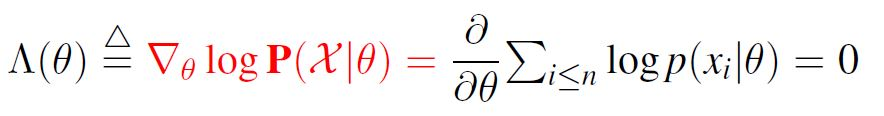
\includegraphics[scale=1]{Figures/ML-Estimator.JPG}
    \label{fig:ML-estimator}
    \end{figure}
\end{itemize}

\textbf{Features of ML-Estimators}
\begin{itemize}
    \item\textbf{Consistent: }$\theta_{ML} \rightarrow$ $\theta_{0}$ in probability as n $\rightarrow \infty$.
    \item\textbf{Asymptotically normal: }$1/\sqrt{n}$ $(\theta_{ML} - \theta_0)$ converges in distribution to a random variable.
    \item\textbf{Asymptotically efficient: }$\theta_{ML}$ minimizes $\mathbb{E}[(\theta_{ML} - \theta_0)^2$ as $n \rightarrow \infty$
    \item\textbf{Equivariance: }If $\hat\theta_n$ is MLE of $\theta$ the $g(\hat\theta_n)$ is MLE of $g(\theta)$
\end{itemize}

\textbf{Cramer-Rao bound: } No estimator reaches expected mean squared error = 0.\\
\quad $\mathbb{E}[(\theta_{ML} - \theta_0)^2 >= \frac{1}{I_n(\theta_0}$ where $I_n$ is the Fisher information. But ML-Estimator is at least asymptotically efficient (reaches bount) (but not necessarily for finite samples!!)

\subsection{Bayesianism vs Frequentism}

\begin{center}
\begin{tabular}{ L{6cm}| L{6cm} }
 Bayesianism  & Frequentism \\ 
 \hline
 -Allows priors  & -Does not allow priors \\  
 -Provides a distribution when estimating parameters  & -Provides a single-point when estimating parameters\\
 -Requires efficient integrastion methods, when computing posteriors. &
 -Requires only differentiation methods, when estimating parameters.\\
 -The prior often induces a regularization term. & -MLE estimators are consistent, equivariant,...\\
\end{tabular}
\end{center}

\textbf{Bias: } $bias(\hat{\theta}_n) = \mathbb{E}[\hat{\theta}_n] - \theta$ The bias measures how much the expected value of the estimator deviates from the true parameter value.

\subsection{Bayesian Learning}
TODO slides 3 p.37

\subsection{Recursive Bayesian Learning}



